\section{Kompilierung zu high-level Architekturen}

\begin{frame}{Wie ein Compiler den AST traversiert}
    \begin{figure}[h]
        \centering
        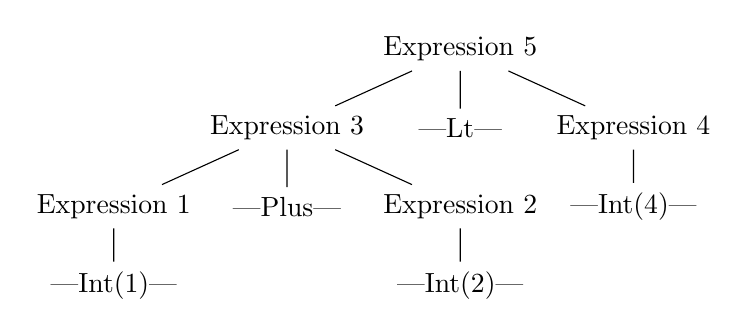
\begin{tikzpicture}[level distance=1cm, sibling distance=2.2cm]
            \node {Expression \encircle{5}}
            child {node {Expression \encircle{3}}
                    child {node {Expression \encircle{1}}
                            child {node {\Verb|Int(1)|}}}
                    child {node {\Verb|Plus|}}
                    child {node {Expression \encircle{2}}
                            child {node {\Verb|Int(2)|}}}}
            child {node {\Verb|Lt|}}
            child {node {Expression \encircle{4}}
                    child {node {\Verb|Int(4)|}}};
        \end{tikzpicture}
        \caption{AST zu \enquote{\texttt{1 + 2 < 4}}.}\label{fig:cmp_simple_tree}
    \end{figure}

    \Lirsting[raw=true, caption={Beispielausgabe zu \enquote{\texttt{1 + 2 < 4}}.}, label={lst:cmp_simple_instructions}, float=H]{deps/paper/listings/simple_compiler_instructions.txt}
\end{frame}

\section{Kompilierung zu WebAssembly}
\begin{frame}{Kompilierung zu WebAssembly}
    \TODO{Write this}
\end{frame}

\section{Kompilierung zu LLVM}
\begin{frame}{Was ist LLVM?}
    \begin{itemize}
        \item Startete als Forschungsprojekt von \emph{Chris Lattner}~\scite{Lattner:MSThesis02}
        \item Neben anderen großen Projekten verwendet auch \emph{Rust} LLVM als sein Backend~\scite[p.~373]{McNamara2021-hz}.
        \item Wird auch von der \emph{Swift} Programmiersprache (Apple) verwendet ~\scite[preface]{Hsu2021-ez}.
        \item Kann aus einer Zwischendarstellung Code erzeugen, der auf der Zielmaschine ausführbar ist
        \item Das Framework ist bekannt für seine aggressiven Optimisierungsmaßnamen
        \item LLVM stellt eine API zur verfügung, mit welcher eine sogenannte \emph{intermediate representation} (IR) erzeugt werden kann~\scite[preface]{Hsu2021-ez}
        \item[\Rightarrow] LLVM ist das backend eines Compilers
    \end{itemize}
\end{frame}

\begin{frame}{Rolle von LLVM in einem Compiler}
    \begin{figure}[h]
		\begin{adjustbox}{max totalsize={\textwidth}{!},center}
            \begin{tikzpicture}[node distance=3mm and 1cm, inner sep=3mm]
                \node (syntactic_analysis_text) [inner sep=0] {syntactical analysis};
                \node (lexical_analysis) [rec, below=of syntactic_analysis_text] {lexical analysis};
                \node (syntactic_analysis) [rec, fit={(syntactic_analysis_text) (lexical_analysis)}] {};

                \node (semantic_analysis) [rec, align=center, right=of syntactic_analysis] {semantic\\analysis};
                \draw [arrow] (syntactic_analysis) -- (semantic_analysis);

                \node (ir_generation) [rec, align=center, right=of semantic_analysis] {LLVM IR\\generation};
                \draw [arrow] (semantic_analysis) -- (ir_generation);

                \node (llvm) [rec, align=center, fill=gray!15, right=of ir_generation] {LLVM\\backend};
                \draw [arrow] (ir_generation) -- (llvm);
            \end{tikzpicture}
        \end{adjustbox}
        \caption{Etappen der Übersetzung mit Verwendung von LLVM}\label{fig:compilation_steps_llvm}
    \end{figure}
\end{frame}
